\chapter{Overall Description}

\section{Product perspective}

The system will be developed from scratch and it will completely replace the legacy system. \newline
It is composed by a client part and a server part.
The latter is composed by an application server (CLup Server) where all the logic is located. It also comprehends the web server, the database server and the mail server,
which all communicate with the CLup Server.
It also has an interface, the API Manager, which exposes the public CLup API, for the QR validation.\todo{External Map API}\newline
The solution for the client part includes two interfaces based on the user type: the mobile app for the customers and the browser for supermarkets' employee and managers.
\begin{figure}[H]
	\centering
	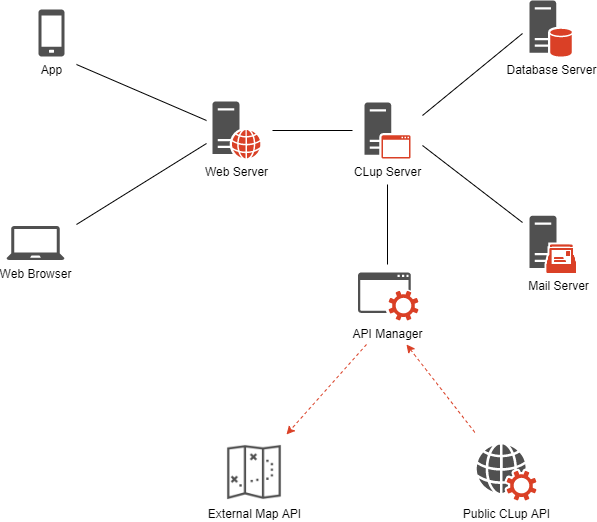
\includegraphics[scale=0.45]{ProdPerspective_Diagram}
	\caption{CLup system diagram}	
\end{figure}	 

\section{Product functions}

\section{User characteristics}

\section{Constraints}

\section{Assumptions and Dependencies}

\subsection{Domain assumptions}
